% !TeX spellcheck = de_DE
\section{Digital Business}
\subsection{What tech is and what it is not}
\begin{enumerate}
	\item Tech is not neutral.
	\item Tech is not inevitable.
	\item Most people in tech want to do good.
	\item Tech history is poorly documented and poorly understood.
	\item Most tech education doesn’t include ethical training.
	\item Tech is often built with surprising ignorance about its users.
	\item There is never just one single genius creator of technology.
	\item Most tech isn’t from startups or by startups.
	\item Most big tech companies make money in just one of three ways (Ads, Big Business, Individuals).
	\item The economic model of big companies skews all of tech.
	\item Tech is as much about fashion as function.
	\item No institution has the power to rein in tech’s abuses.
\end{enumerate}

\subsection{Plattform Geschäftsmodelle}
\begin{itemize}
	\item Starke Zunahme
	\item Funktionsweise über Software-Angebot
	\item Funktionsweise über Sammeln, Übertragen, Auswerten und Monetarisieren von persönlichen Daten.
	\item Direkte und indirekte Netzwerkeffekte: Nutzerwachstum und Wachstum der Nutzer der anderen Seite (z.B. Videospieler und Spieleentwickler). Selbstverstärkender Wachstumseffekt (exponentiell)
	\item Plattform-Geschäftsmodelle sind heute nicht nur dominant in den Bereichen	Social Media, Reisen (Buchung und Bewertung), Literatur und Musik, sondern inzwischen auch in den Bereichen Transportwesen, Banking, Gesundheitswesen, Energie, etc. = von B2B zu B2C
	\item Weltweites Phänomen auf
	\begin{itemize}
		\item globaler (Amazon, Apple, Google, Alibaba, Facebook)
		\item nationaler Ebene (z.B. Rakuten-J, Delivery Hero-D, Naspers-SA, Flipkart-Ind, Javago-Nig)
	\end{itemize}
	\item Plattform-Ökosysteme verändern die Unternehmenslandschaft durch die Digitalisierung von Produkten, Leistungen und Prozessen.
	\item Plattform-Geschäftsmodelle erhöhen Produktivität:
	\begin{itemize}
		\item effizientes Matching von Personen (eBay, LinkedIn, etc.)
		\item effiziente Nutzung von Gegenständen (Immobilien, Autos, Arbeitsplätze, etc.)
	\end{itemize}
	\item Plattform-Geschäftsmodelle bringen Innovationen hervor, z.B. 9 US-Plattformen haben 11’585 Patente im Jahr 2014 angemeldet.
	\item Viele “Unicorns” (Unternehmen mit Marktkapitalisierungswert von über einer Milliarde) sind Plattform-Geschäftsmodelle.
	\item Plattform-Geschäftsmodelle sind disruptiv, d.h. sie greifen bestehende Industrien (Bankenwesen, Transportwesen, Fernsehen, etc.) an.
	\item Kontroverse Diskussion über Regulierung (z.B. in der Schweiz: AirBnB, Uber, Booking) in Bezug auf Wettbewerbsverzerrung, Steuern, Versicherungen, Preisverzerrung von Löhnen, etc.
	\item Tendenz zu Oligopolen (horizontale Integration) vs. Monopson (grosse Zahl von Anbietern stehen nur einem Nachfrager gegenüber, vertikale Integration)
\end{itemize}

\subsubsection{Attribute}
Informationen bzw. Gegenstände sind kostenlos, perfekt und unmittelbar verfügbar
\begin{itemize}
	\item \textbf{Kostenlos:} «First Copy Costs» Speicherplatz / Übermittlung / Reproduktion => Grenzkosten gegen 0
	\item \textbf{Perfekt:} Jede digitale Kopie ist eine perfekte neue Produktion des Originals.
	\item \textbf{Verfügbar:} Sobald ein Netzwerk verfügbar ist, können die perfekten und kostenlosen Gegenstände ohne bzw. mit geringer Verzögerung von einem zum anderen Ort übermittelt werden.
\end{itemize}

\subsection{Netzwerkeffekt}
\begin{itemize}
	\item Im Laufe der letzten Jahre wechselten Mobilfunknutzer zunehmend für das Versenden von Nachrichten zu WhatsApp.
	\item Folge: die meisten Kontakte der Mobilfunknutzer verwenden bereits WhatsApp und die Nutzung wird zunehmend zur sozialen Norm .
	\item Dienstleistungen werden für jeden Nutzer wertvoller, je mehr Menschen sie nutzen.
	\item Mit zunehmender Beliebtheit der App fühlten sich die SMS-Nutzer zunehmend ausgeschlossen, so dass sie der alten Nachrichtentechnologie eher den Rücken zukehren. Dies verstärkt den Netzwerkeffekt.
\end{itemize}

\subsection{Transaktionskosten}
\begin{itemize}
	\item Ob eine Transaktion stattfindet ist abhängig davon:
	\begin{itemize}
		\item Aufwand, geeigneten Geschäftspartner zu finden (Informationskosten),
		\item Vertrag abzuschliessen (Verhandlungs- und Vertragskosten),
		\item ggf. nachträgliche Vertragsanpassungen durchzuführen (Anpassungskosten)
		\item Erfüllung der vertraglichen Leistungen zu kontrollieren bzw. durchzusetzen (Kontroll- und Durchsetzungskosten).
	\end{itemize}
	\item Transaktionskosten haben grossen Einfluss, ob bestimmte ökonomische Aktivitäten stattfinden.
	\item Digitaler Fortschritt verändert Transaktionskosten: Erfolgreiche neue Geschäftsmodellansätze digitaler Plattformen nutzen die Transaktionskostensenkenden Potenziale digitaler Technologien in hohem Masse. => Veränderungen bei den bestehenden Marktbeziehungen
	\item Wenn durch Leistungsangebot Transaktionskosten signifikant gesenkt werden, kann sich Plattformanbieter als Intermediär zwischen den Marktteilnehmern etablieren und so die Marktbeziehungen fundamental ändern.
	\item Plattformen koordinieren das Gesamtsystem, stellen die Interoperabilität innerhalb des Gesamtsystems sicher und reduzieren die Transaktionskosten (Koordinationskosten) für die mit dem Ökosystem der Plattform verbundenen Akteure.
\end{itemize}

\subsection{Klassifikation}
\begin{multicols}{2}
	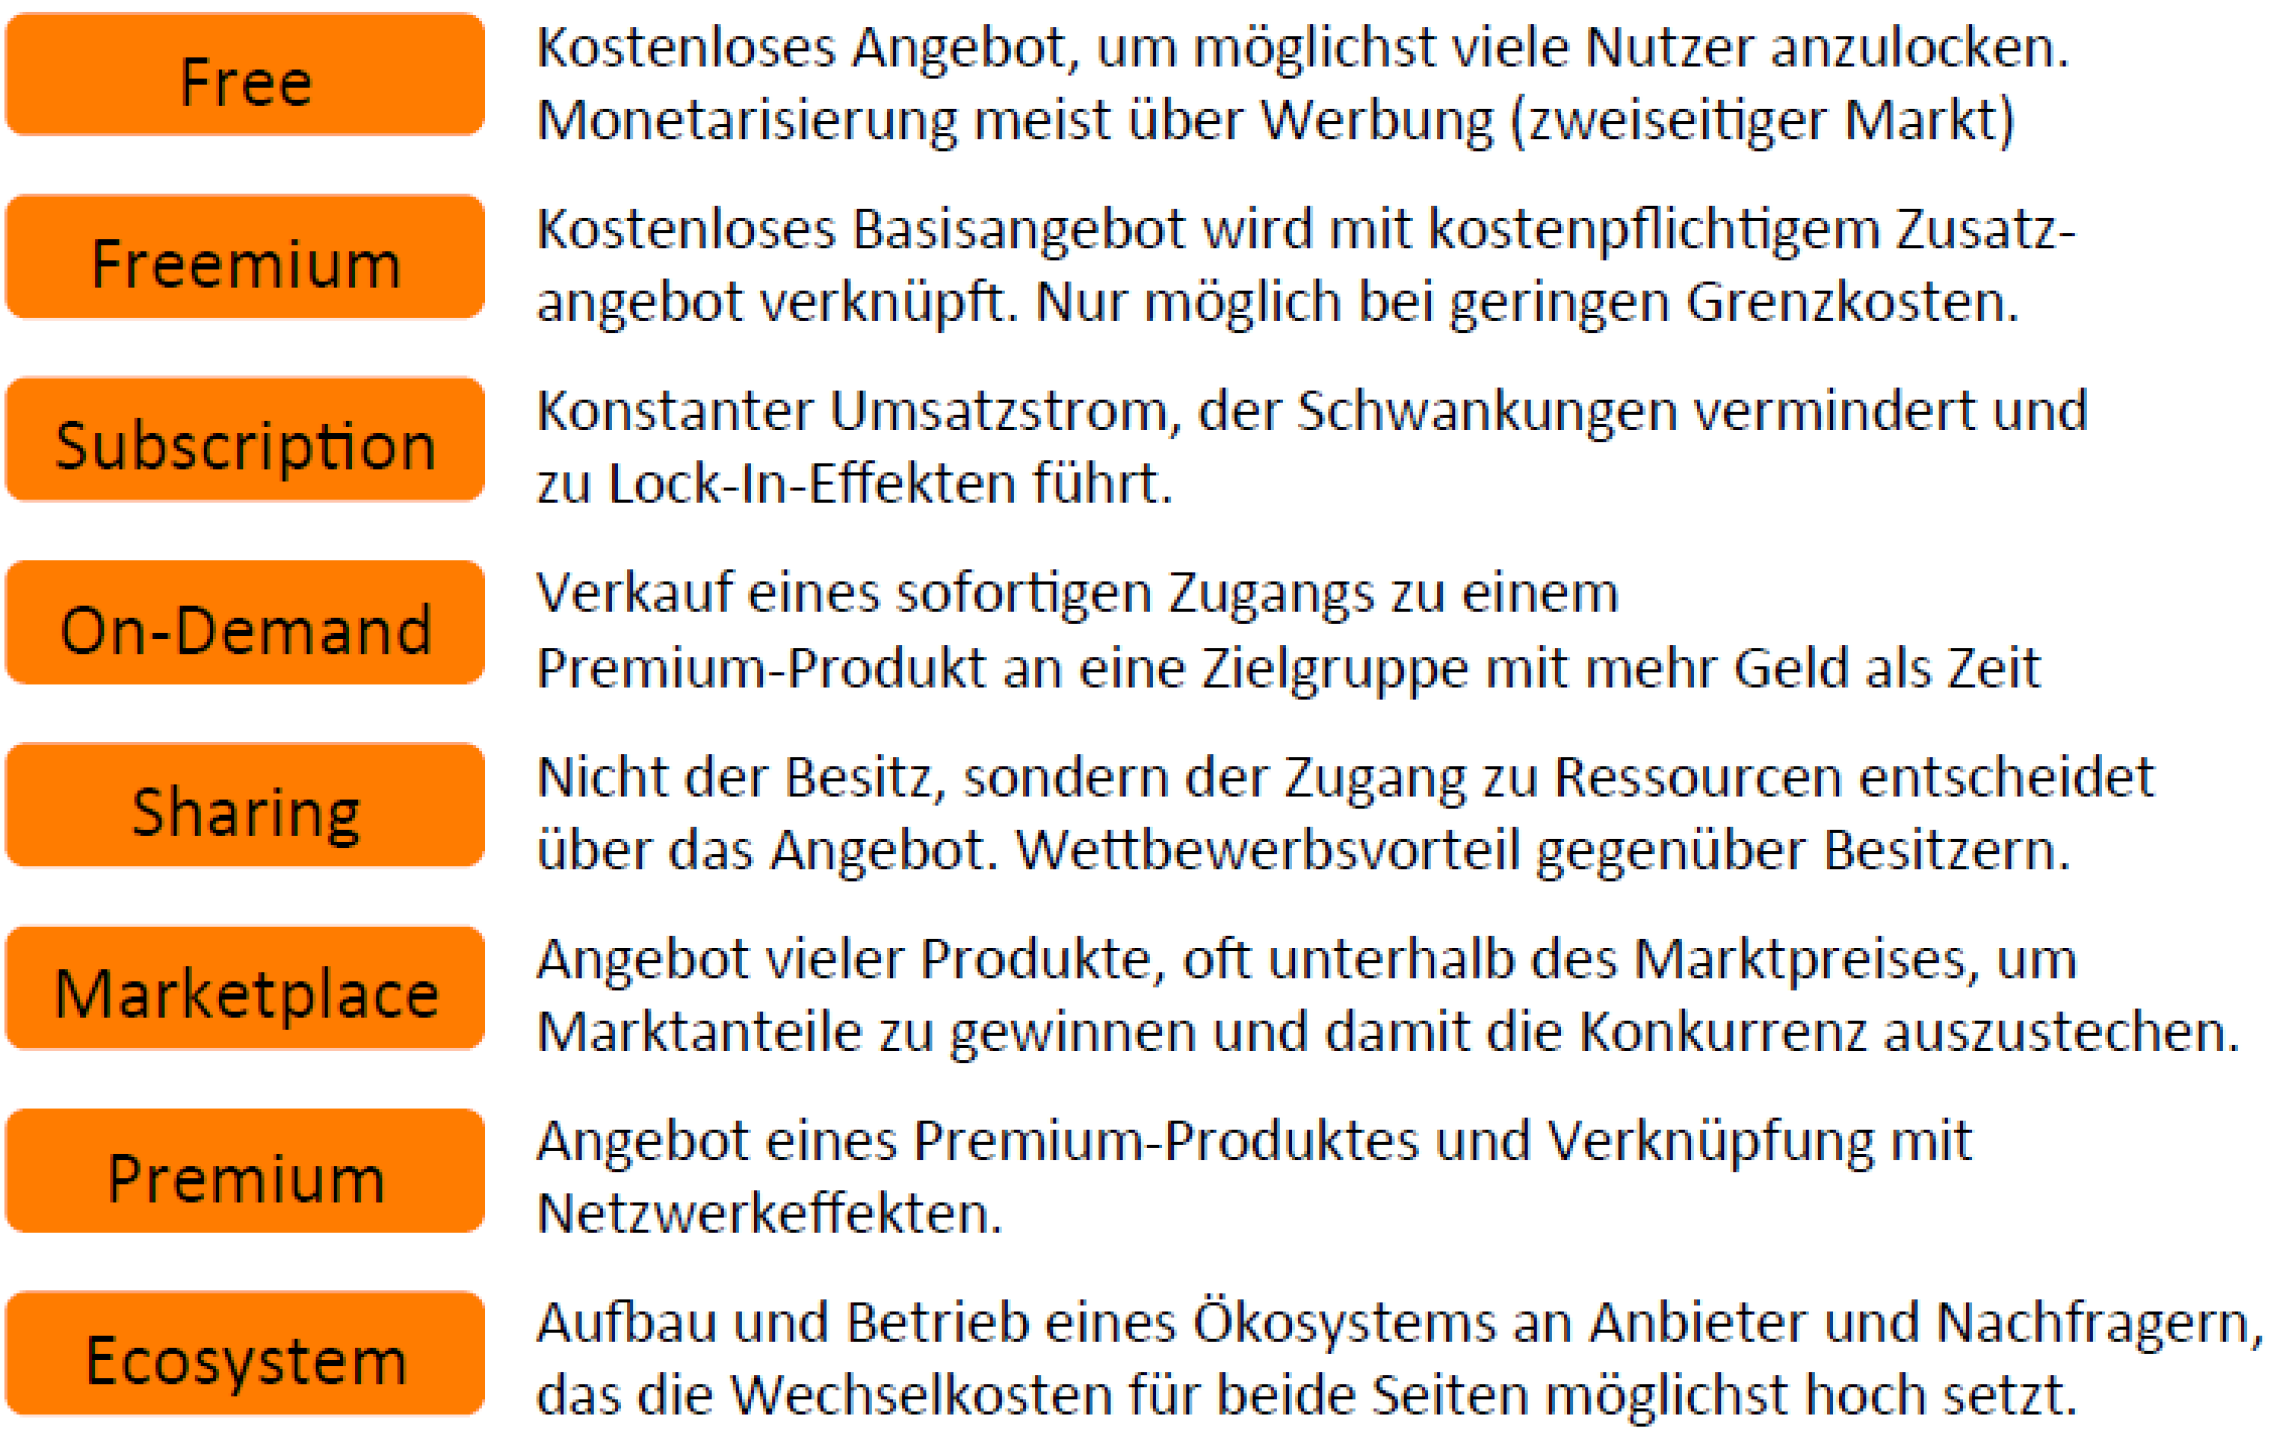
\includegraphics[width=1\linewidth]{images/klassifikation}
	\begin{itemize}
		\item Multi-sided Platform
		\item Razor and Blade (Basisprodukt sehr günstig, Zusatzprodukt sehr teuer)
		\item Free Trial
		\item Long Tail (mit 20\% der Produkte werden 80\% der Einnahmen generiert)
	\end{itemize}
\end{multicols}

\subsection{Unbundling, Rebundling}
\textbf{Unbundling:}
\begin{itemize}
	\item Trennung von einzelnen Produkten/Leistungen verstanden, die eng miteinander verknüpft sind/waren.
	\item Beispiel: iTunes von Apple. Die von Apple bewirtschaftete Plattform iTunes ermöglicht den Kunden den Kauf von einzelnen Liedern und verpflichtet nicht, ein gesamtes Album zu kaufen. Die kostenpflichtigen Lieder sind dabei unmittelbar verfügbar.
\end{itemize}
\textbf{Rebundling:}
\begin{itemize}
	\item beschreibt das neue (Wieder-)Zusammenstellen von einzelnen Leistungen.
	\item Beispiel: Spotify/Streamingdienste (Mix der Woche). Streamingdienste bieten der Kundschaft eine grosse Medienbibliothek an. Die Musik steht den Kunden jederzeit perfekt, frei und unmittelbar zu Verfügung. Für die Nutzung der Streamingdienste zahlen die Nutzer eine monatliche Nutzungsgebühr.
\end{itemize}

\subsection{O2O-Plattformen}
\begin{itemize}
	\item Sonderform: Online-to-offline Plattformen (O2O)
	\item In Bereichen Transportwesen, Unterkunft, Shopping, etc. => Handel mit	physischen Gütern und Leistungen.
	\item Mit Inventar, das begrenzt haltbar / verfügbar ist => Marginalkosten, aber Kapazitätsgrenzen ($\neq$ kostenlos, perfekt, verfügbar)
	\item Leistungen: Auto waschen, Wäscheservice, Kochservice, Essenslieferung, Massage und Maniküre, Hotelbuchung, locale Discounts, etc., die zu bestimmer Zeit an einem bestimmten Ort gebucht werden können.
	\item Betrieber nutzen “Revenue Management”-Techniken um den Match zwischen Angebot und Nachfrage zu verbessern.
	\item Beispiele: ClassPass, Postmates, Lyft, Uber Airbnb, Grubhub, Caviar, etc.
	\item Hauptsächlich Konsumentenorientiert, aber B2B O2O entwickelt sich weiter, z.B. Flexe.
	\item Schnelle Arrangements an Transaktionen durch Zugang zu grossem Netzwerk an Kunden
	\item Vorreiter: China
\end{itemize}

\subsection{Angebot und Nachfrage}
\begin{multicols}{2}
	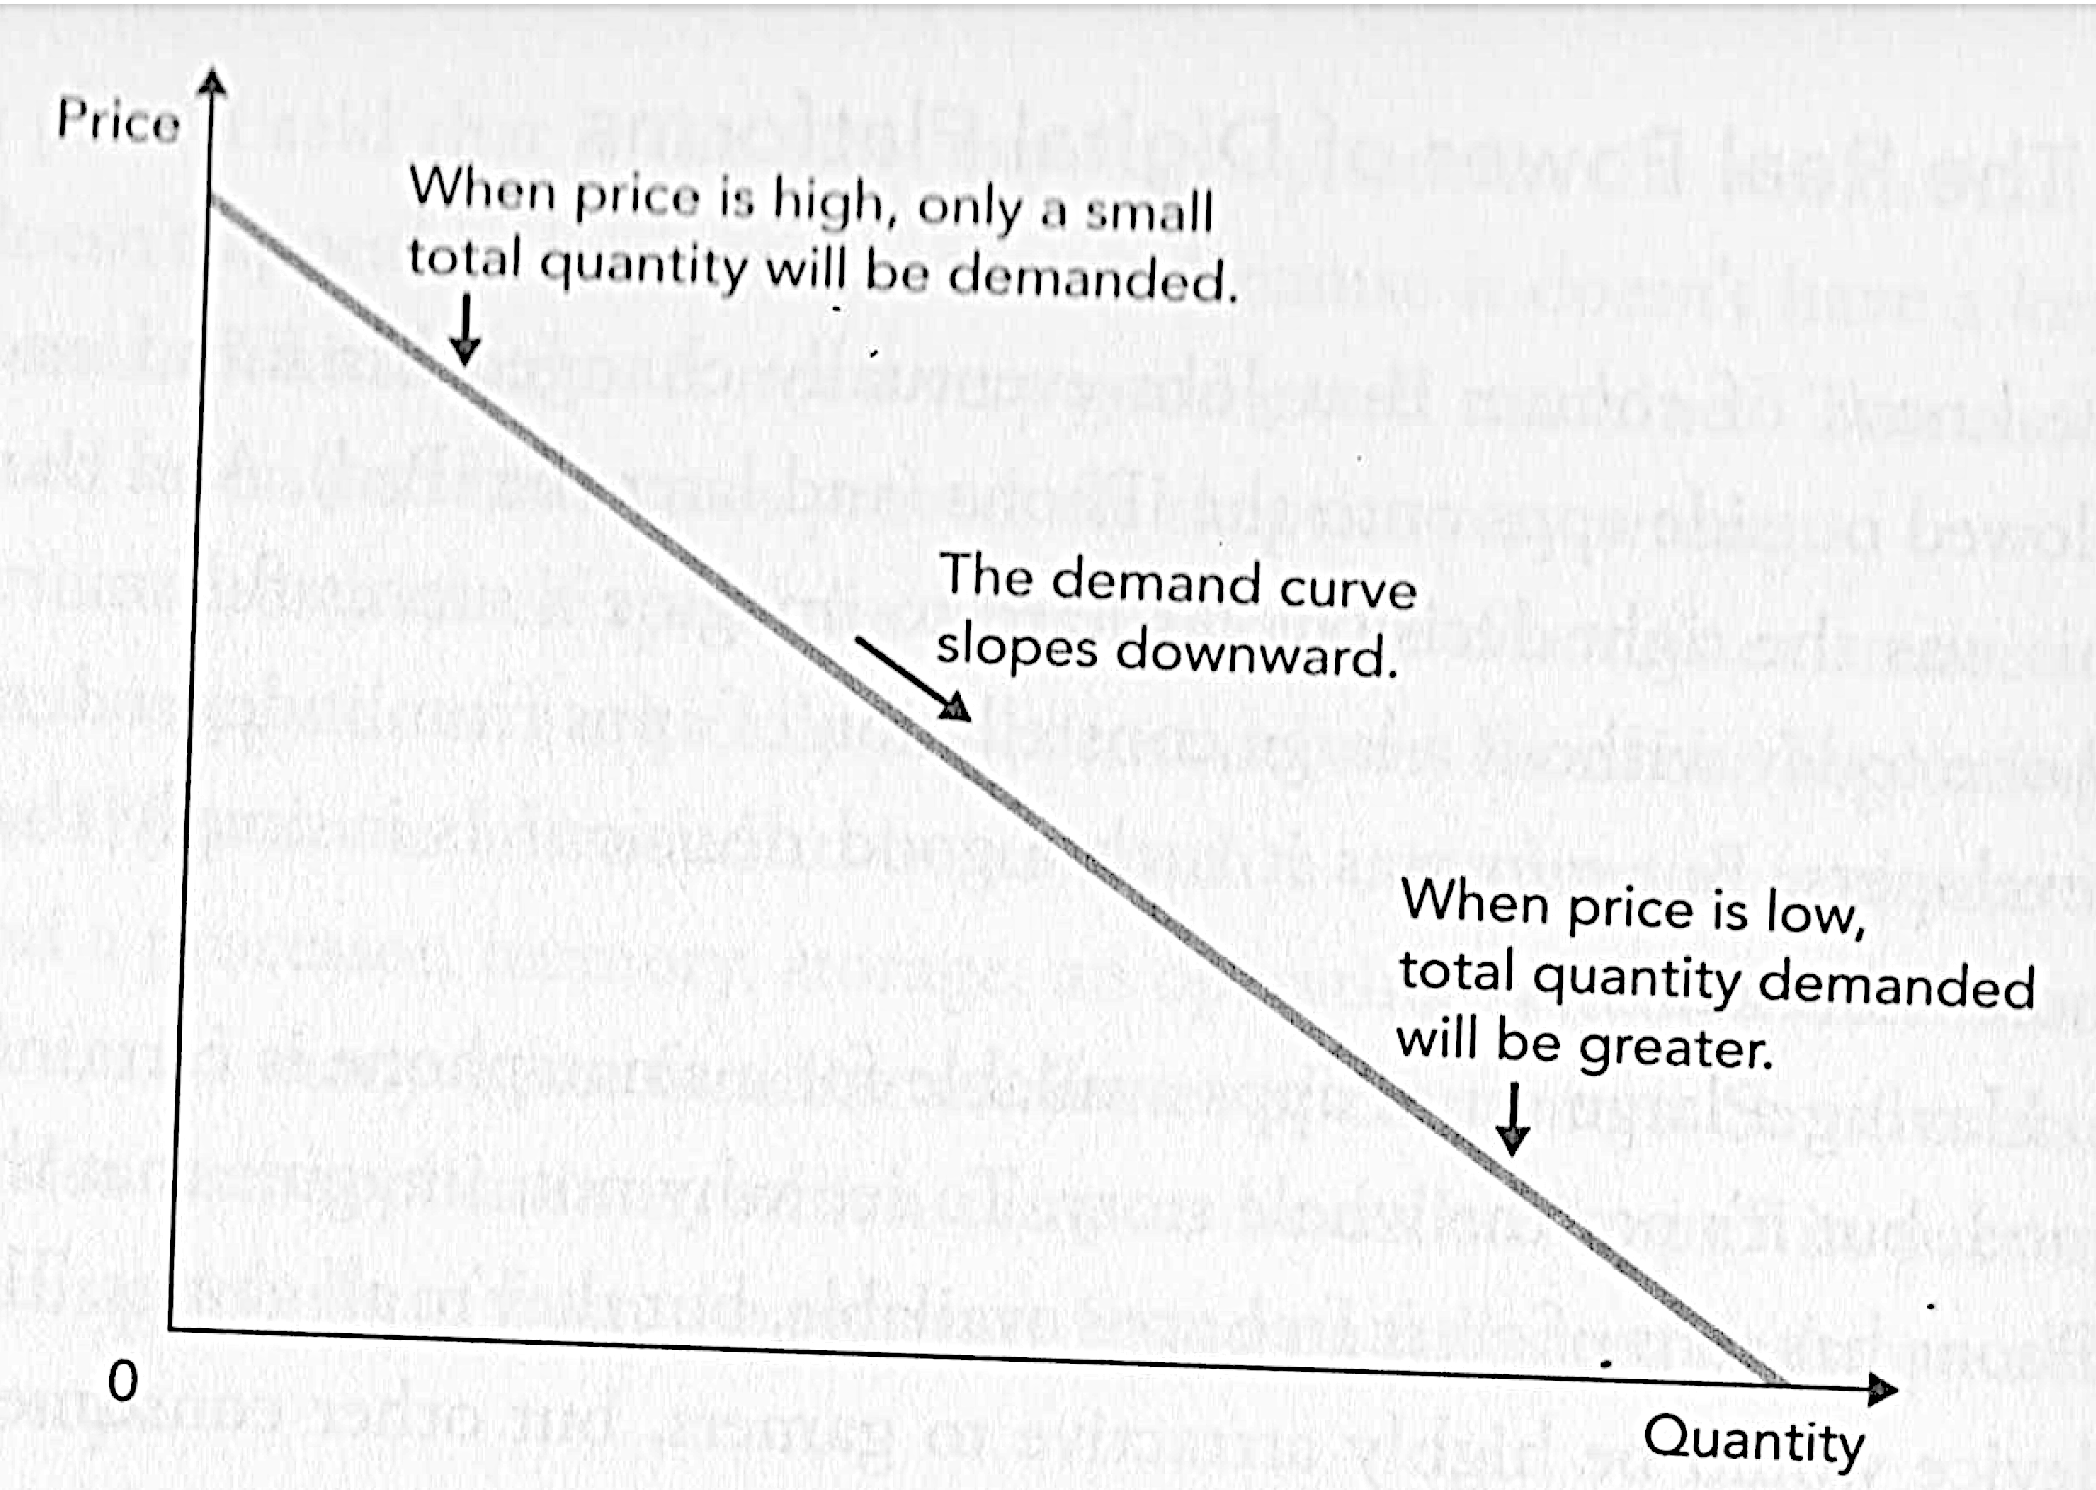
\includegraphics[width=1\linewidth]{images/angebot_nachfrage_1}
	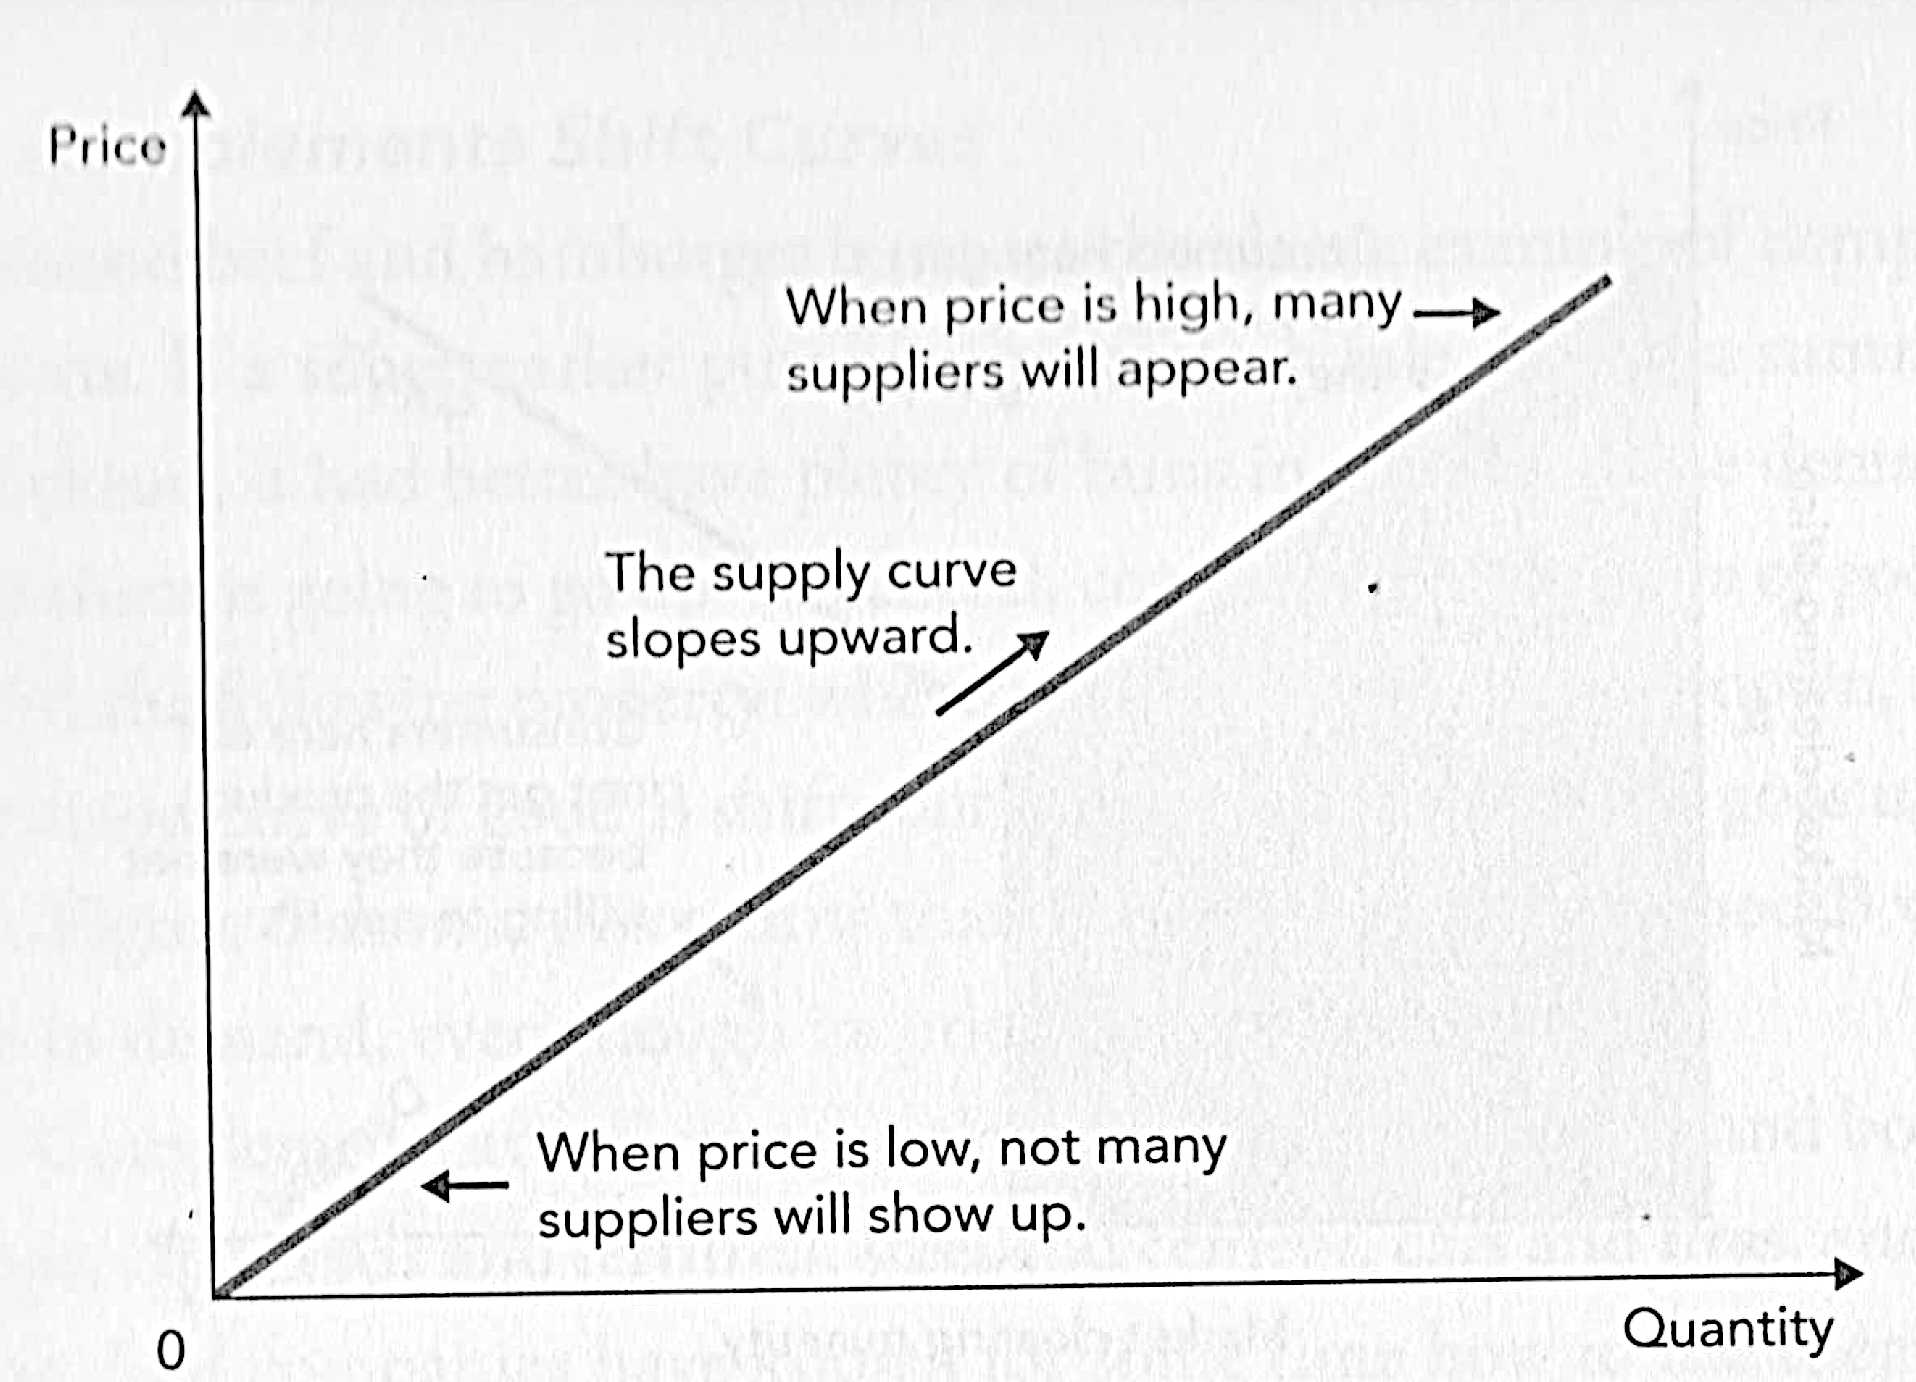
\includegraphics[width=1\linewidth]{images/angebot_nachfrage_2}
\end{multicols}

\subsection{Komplementäre Produkte}
\begin{multicols}{3}
	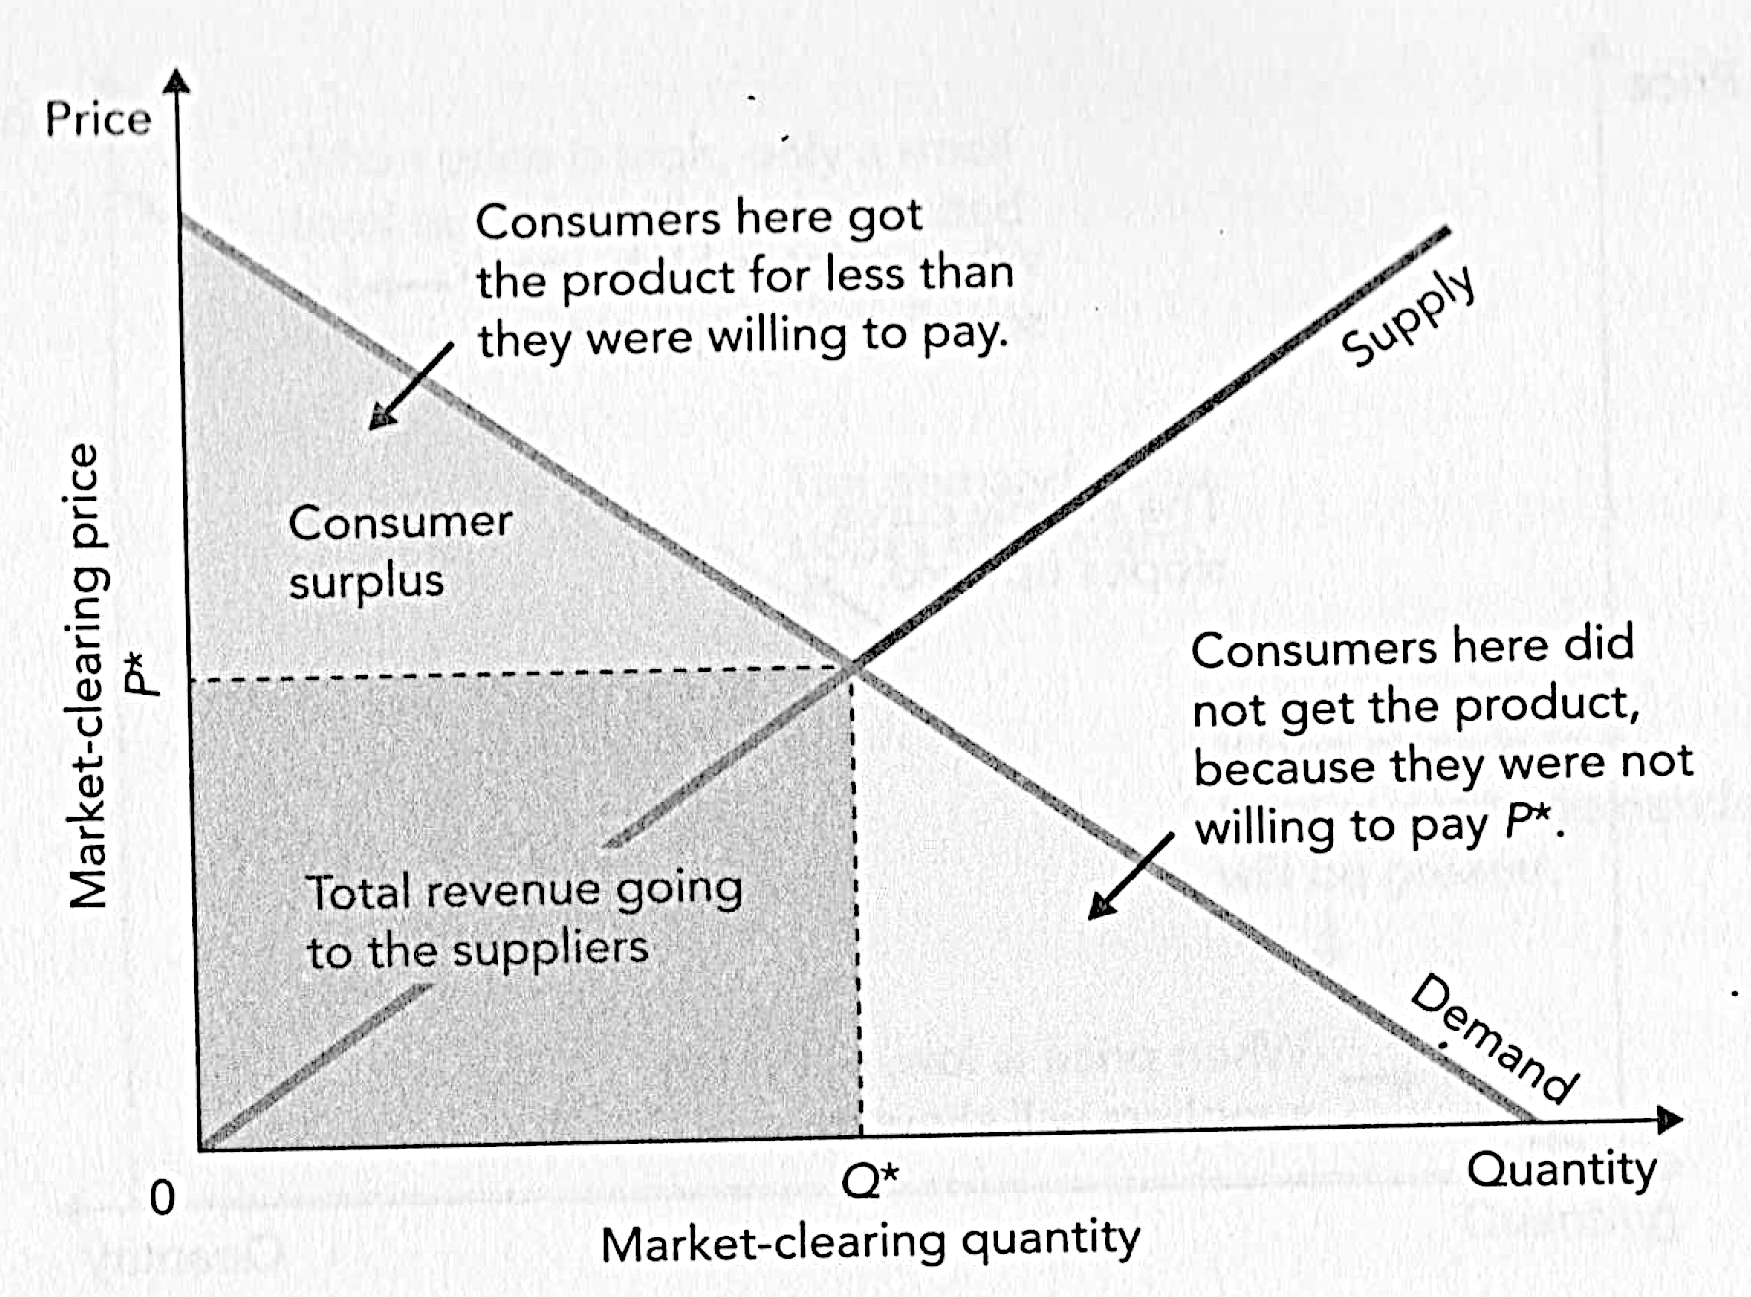
\includegraphics[width=1\linewidth]{images/komp_produkte_1}
	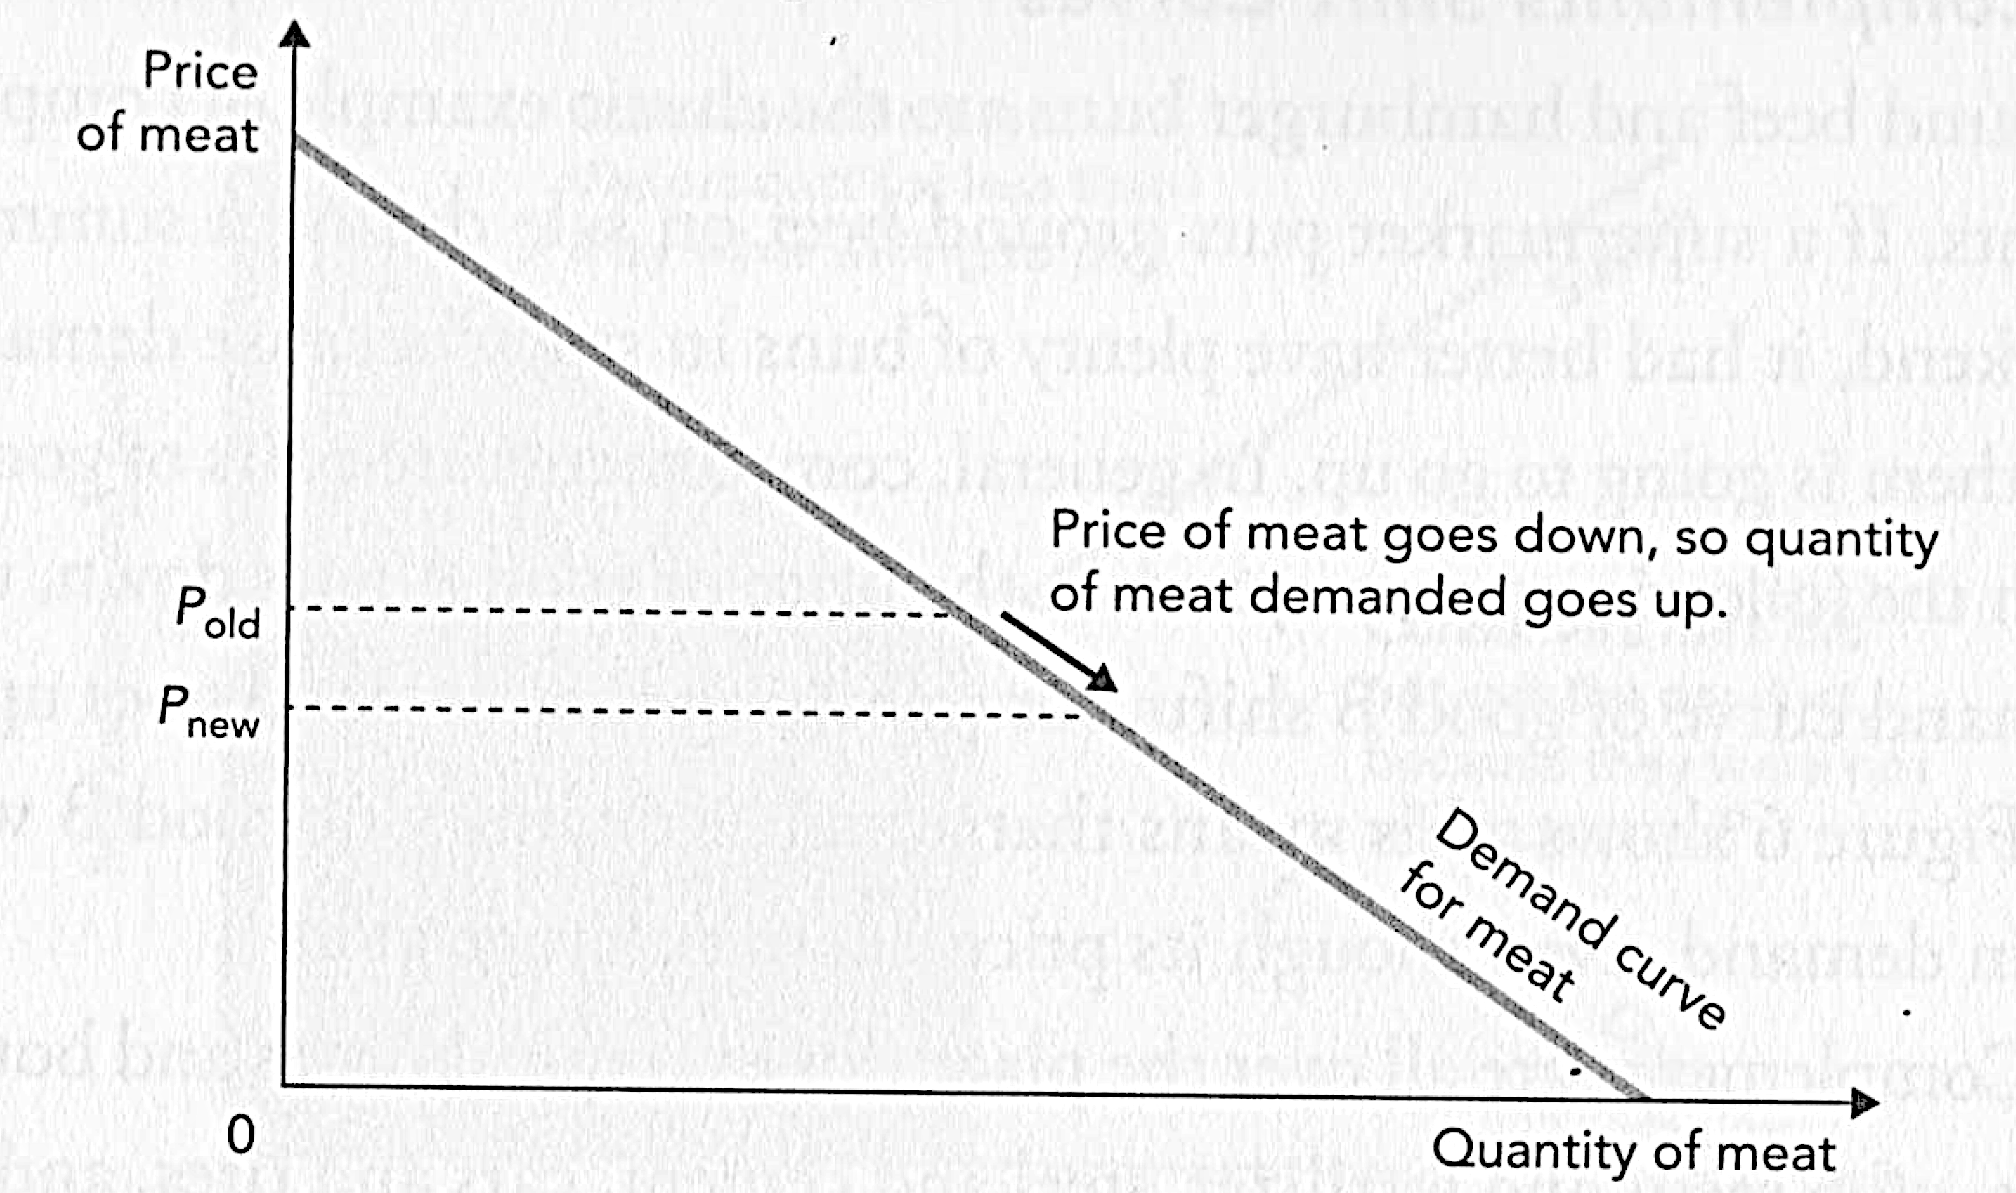
\includegraphics[width=1\linewidth]{images/komp_produkte_2}
	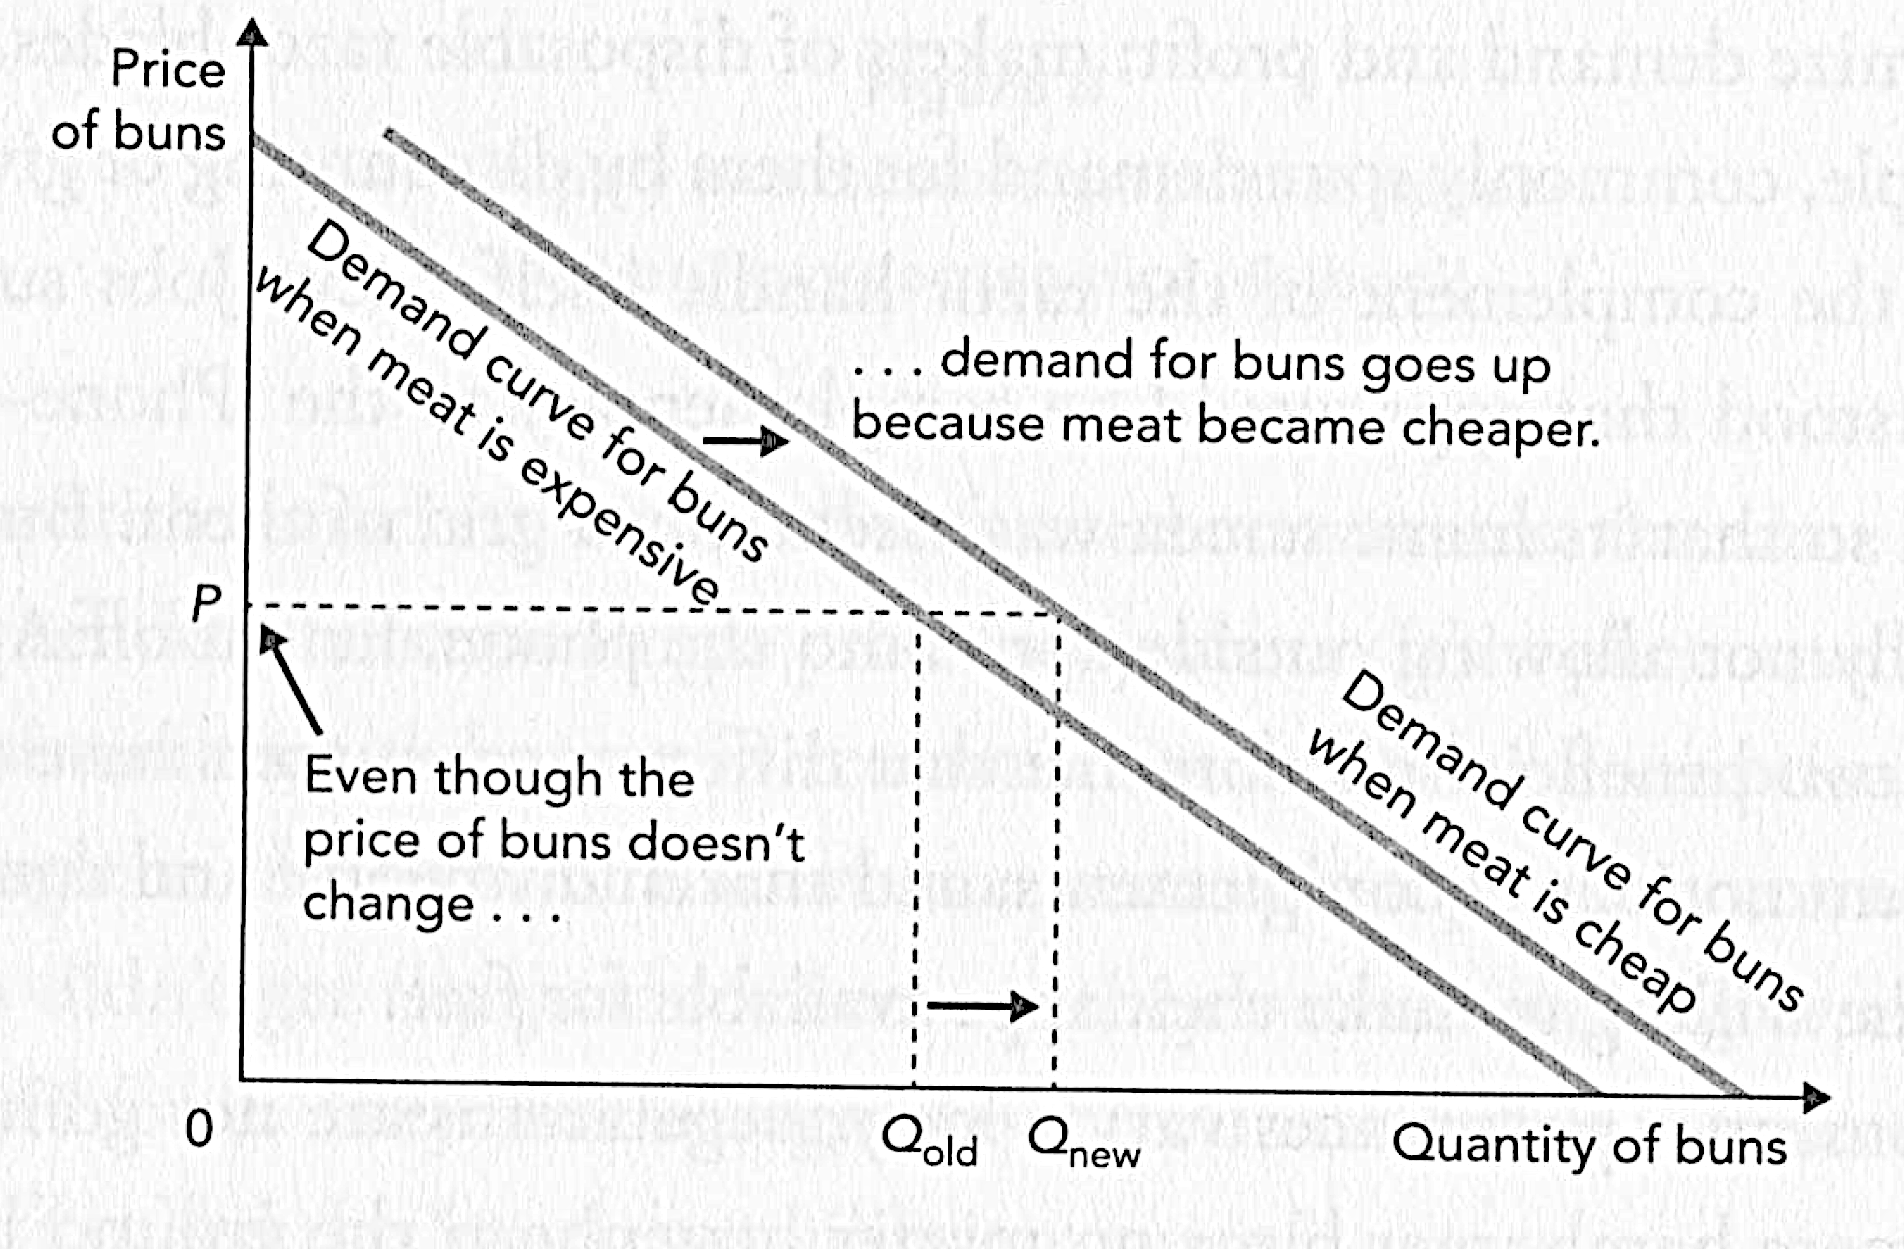
\includegraphics[width=1\linewidth]{images/komp_produkte_3}
\end{multicols}

\begin{itemize}
	\item Complements are goods that can be used with another good. They are also called paired goods.
	\item The classical example for a paired good and to explain how complements shift curves is ground beef for hamburger patty and hamburger buns. If a shop decides to offer the ground beef at a discounted price the demand for hamburger buns will rise naturally, even if the price for them stays the same. This will result in a shift of the demand curve of hamburger buns.
	\item Two products are complements if a drop in the price of one pushes out the demand curve for the other.
	\item When a platform is opened up to allow outside contributions, its owners realize an important benefit: demand for the owner’s product goes up as others contribute complementary goods. When these complements are digital, many of them will be free, perfect and instant.
\end{itemize}
\pagebreak
\begin{multicols}{2}
	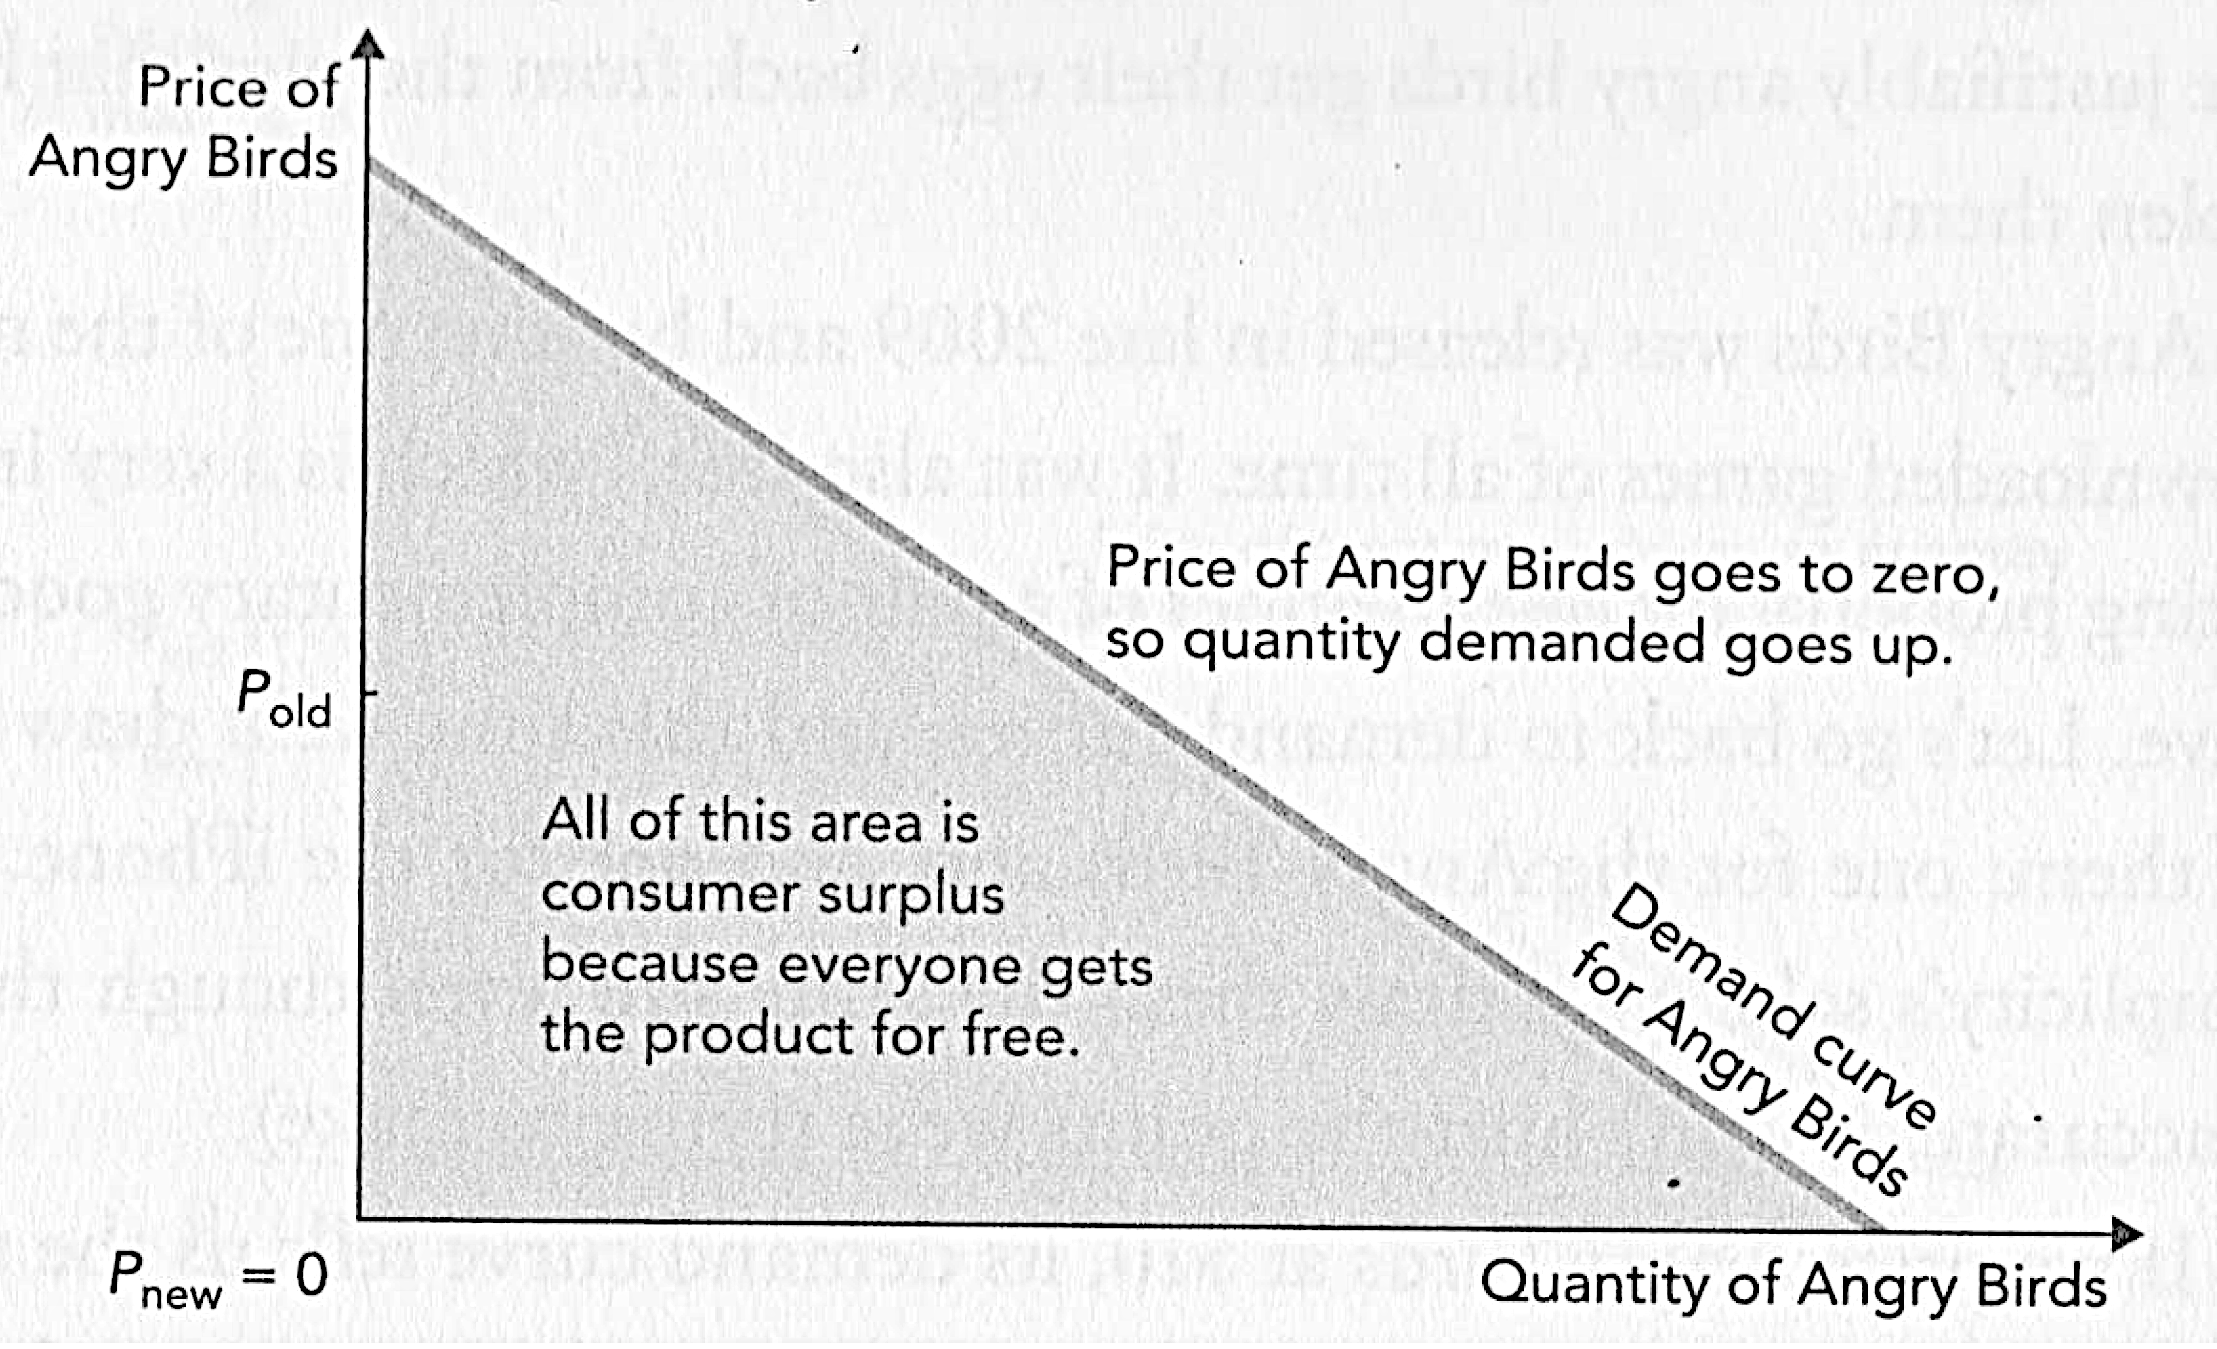
\includegraphics[width=1\linewidth]{images/komp_produkte_4} 
	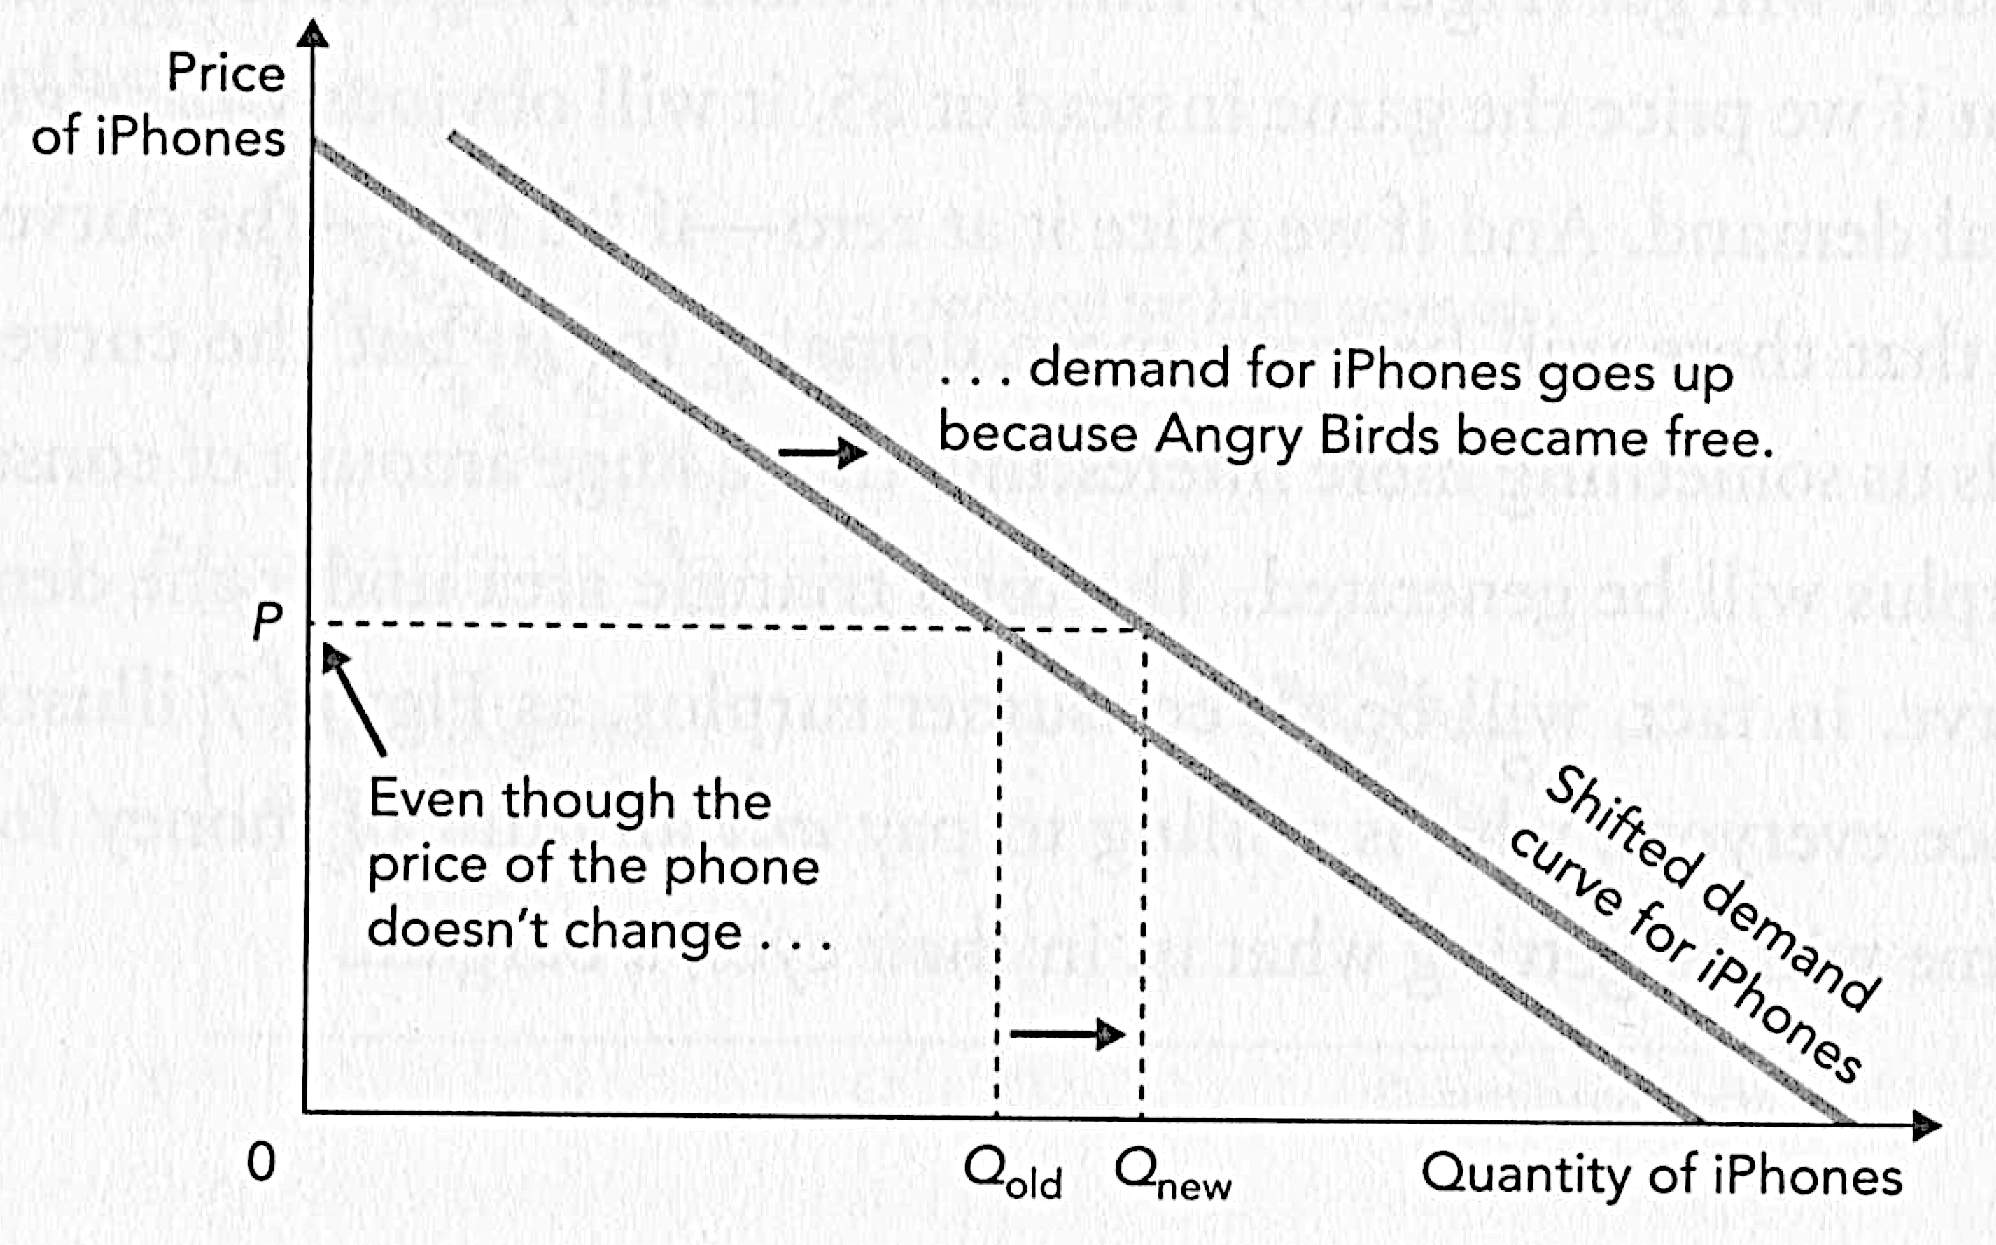
\includegraphics[width=1\linewidth]{images/komp_produkte_5}
\end{multicols}

\begin{itemize}
	\item Platform owners often have to curate contributions from outsiders to maintain standards (e.g. apps on the iPhone).
	\item Example: Apps are an open marketplace, where everyone can create an app and upload it to a platform from where consumers can download it.
	\item Apple’s incentive to open the Appstore to independent app developers, was to cater the needs of more customers. The independent app developers with “Freemium” businesses offer their initial product for free and will subsequently
	charge customer for add-ons.
	\item Free versions of apps will spur sales of the more extended paid-for versions of the apps. Revenue can be made by offering ad space in their apps, public services can be improved with the help of apps and paired products can generate more sales when backed by an app.
\end{itemize}